\documentclass[10pt,article]{IEEEtran}
\usepackage{cite}
\usepackage[cmex10]{amsmath}
\usepackage{array}
\usepackage{url}
\usepackage{graphicx}
\usepackage{graphics}
\usepackage{verbatim}
\usepackage{lmodern}
\usepackage{flushend}
\begin{document}
\title{Toolset for an automated troubleshooting in SDNs}

\author{\IEEEauthorblockN{Knop Thibaut, Rochet Florentin\\}
\IEEEauthorblockA{EPL,
UCL\\
Louvain-la-Neuve, Belgique\\
\{thibaut.knop,florentin.rochet\}@student.uclouvain.be}}


\maketitle
\begin{abstract}
In this paper, we propose a methodological review of the existing tools designed for Software-Defined networks troubleshooting. This review is organized using the SDN layering architecture, and aims to show the possibility of an automated localization of the bugs in the different layers of SDN. The toolset presented here allows administrators to more focus on fixing than localizing issues. We will go through the layers by choosing the most significant and relevant tools for each (pair of) layer(s) we are considering, regarding other existing tools : NDB for spotting incoherences between policies and their effects, VeriFlow for verifying invariants in real-time, SOFT for spotting bugs in OpenFlow switches configuration, NICE either for the switch firmware of the controller software and FlowChecker supporting verification for different OpenFlow federated infrastructures.
\end{abstract}

\begin{IEEEkeywords}
OpenFlow, SDN, Troubleshooting, Layer, Controller, Consistency, Model-checking, Verification
\end{IEEEkeywords}

\section{Introduction}

For many years, the debugging has always been one of the major concerns in network maintenance. In order to localize problems into the network, operators usually use a narrow toolset, composed of traditional tools as \verb@ping@, \verb@traceroute@ and \verb@SNMP@ agents\cite{zeng2012automatic}.\\
Hopefully, this difficult and time-consuming\cite{zeng2012automatic} process could change, given the deployment of Software-Defined Networks. In a nutshell, SDNs are based on the separation between control- and data planes, which offer the opportunity of programmable networks\cite{mckeown2008openflow}. Those SDNs are composed of a network of switches managed by a logically-centralized controller, whose role is to (un-)install rules into the flow table of the switches, to read traffic statistics and respond to the network activity.\\
However, and because SDNs allows different operators and developers to dynamically program the same network, the complexity of software will increase\cite{Sherwood:2010:PNT:1924943.1924969} and potentially the numbers of bugs.
To minimise the trade-off between introducing new functionality and  increase the number of bugs in the network, there is a serious need for a complete and effective automated testing toolset, allowing the admins to focus on fixing the issues instead of localizing them. In traditional network architecture, it is almost impossible to create such an automated test suite, due to the complexity of \textit{"knowing the operator's intent"} and \textit{"checking network behavior against intent"}\cite{Heller:2013:LSL:2491185.2491197} (for more information about how traditional networks could be extended to support automated troubleshooting, please refer to \cite{Heller:2013:LSL:2491185.2491197}).\\
As we will explain (see Section~\ref{layering}), we use the different layers of the SDN stack to review the available tools for automated troubleshooting. Note that the methodology and the structure of this paper is influenced from the one used in\cite{Heller:2013:LSL:2491185.2491197}. It indeed seems the better way to articulate and present the different tools destined to localize the problems and their cause in an automated way.
The paper is structured as follow : first we recall the different layers of the SDN stack, and how it can be leveraged to provide automated troubleshooting for SDNs, then we present different existing tools by positioning them regarding the SDN layering, and we eventually conclude.

\section{SDN layering, the key used to an automated troubleshooting}\label{layering}
 % Expliquer ici la stack SDN (decomposition en layer) et donner l'intuition concernant la plus grande facilité pour remonter à l'origine d'un probleme.
Finding and solving network bugs are not the aim of SDN, but we can use it to re-think the way we troubleshoot networks.\\ The SDN architecture is decomposed into  layers, those layers can be represented in a two dimensionnal array. As you can see on Figure \ref{layers}, we have the two main layers called \textit{State layers} and \textit{Code layers}. The state layers hold a representation of the network configuration for each parts of the network architecture. The code layers implement logic to maintain the mapping between two state layers. Each state layers should verify the equivalence properties, which means that each of them should correctly mapping every other state layer. The idea is that, for each policy, if the state layers are correctly mapped among each other, then the policy is  set and acts like it should.\\
On the Figure \ref{layers}, you have the following elements:\\
\textbf{Policy} - Policies are set up by the network administrator to configure the Logical View. These policies can be routing, access control or QoS policies. They are written inside a control application. See \cite{OpenStack_Quantum} for exemple.
\\
\textbf{Logical View} - Abstract representation of the network which aims to make things easier for the control application to create policies. A mapping between the Logical View and one or more Physical View are done by Network Hypervisor.\\
\textbf{Physical View} - This is a correspondance with the real network element, a representation of it handled by the network OS. The protocol used to configure the network element is one like OpenFlow \cite{OpenFlow}. A physical View has thus a one-to-one mapping with a real network element.
\\
\textbf{Device State} - State of the network element maintened by its firmware.
\\
\textbf{Hardware} - Network element. \\

Thanks to the SDN stack, one can first build a tool to check consistency between state layers in order to identify on which part of the network architecture a bug is happening (in which \textit{code layer}). Then, when the layer is identified, an other tool take over to localize the issue inside the code layer. We will see in section \ref{Network Troubleshooting - Tools} which kind of tools could be used to handle this bug hunting. Tools to find the code layer concerned by the issue and tools which operate inside the code layer, to find the cause of the bug.

\begin{figure}
\centering
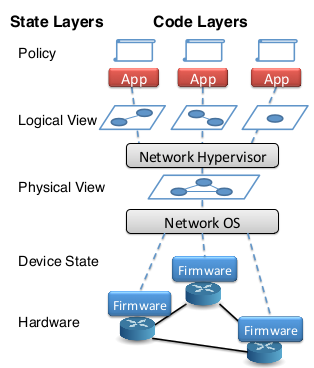
\includegraphics[scale=0.60]{layers.png}
\caption{SDN architecture\label{layers}\protect\footnotemark}
\end{figure}
\footnotetext{Source : \cite{Heller:2013:LSL:2491185.2491197}}
\section{Network Troubleshooting - Tools}
\label{Network Troubleshooting - Tools}
\subsection{Network Debugger (NDB)}
SDNs bring a new way of building networks: like a programmer build a software, a network administrator will be able to program its network. The software programmer has tools to debug its program, like the well-known GDB.\\
NDB is a tool inspired from GDB, it aims at finding network error by identifying incorrect sequence of events. NDB has the ability to do a sort of \textit{breakpoint}, which is in fact a packet filter. When packet are matched by this filter, the breakpoint is triggered and the entire trace of that packet is displayed. The authors mention that the term \textit{tracepoint} should be more appropriate but the term \textit{breakpoint} is more familiar. NDB uses its \textit{backtrace} primitive to show the sequence of events for a packet. This trace is simply the sequence of forwarding actions applied on the packet by the switches through which it passed. For example of NDB utilisation, please refer to its paper \cite{ndb_paper}.\\
In our layering SDN architecture, NDB give us the opportunity to build a tool to confirm the right action of the policies implemented in the control application. For example, if a routing bug occurs in the network, a tool of top of NDB could observe paths taken by packets and complete switches states in order to conclude if the policies are correctly matched or not. If the policies are correctly matched, it means that the network administrator has written policies that dont't fit his needs. In this case, NDB has found the \textit{code layer} where the issue happen. Now if the policies are not correctly matched, then the issue does not come from an incorrect implementation. NDB has thus exclude the implementation to be the root of the bug and the search can continue among other layers, with other tools such as SOFT\cite{SOFT}.

\subsection{VeriFlow}
If the actual behavior of the network does not correspond to the policy, then the issue can potentially be found in the erroneous correspondance between the Policy \textit{state layer} and the Device State \textit{state layer}. There exist different tools to verify this hypothesis. The one we discuss here have the advantage to verify some network invariants in real-time. Other tools as Anteater and Header Space Analysis (HSA) that are also used in the same purpose carry out the static analysis of snapshots of the network data-plane state\cite{Kazemian:2012:HSA:2228298.2228311}\cite{Mai:2011:DDP:2018436.2018470}. Since SDN controllers are capable of installing around 30.000 flows per second while maintaining less than 10 ms delay for the installation, it is absolutely not enough to have tools that check for network invariant with a latency of the order of seconds \cite{Khurshid:2013:VVN:2482626.2482630}.\\
VeriFlow acts as a proxy in between the SDN controller and the switches and this proxy verifies some common network invariants at each forwarding rule installation with a very high speed. In order to achieve a 7ms delay inflation with regards to traditional TCP connections\footnote{Test configuration : 20 nodes OpenFlow network sing Mininet and a NOX controller\cite{Khurshid:2013:VVN:2482626.2482630} }, VeriFlow slices the network into equivalences classes, then builds a virtual forwarding graph for each ones using a trie structure, and finally checks invariants by traversing those graph with a depth-first search approach. Note that VeriFlow allows to spotting network issues before they reach the network, which is very valuable.\\
As limitations, we can note that presently, VeriFlow only checks for reachability invariants, and that it is not suitable for multiple/distributed controller \cite{Khurshid:2013:VVN:2482626.2482630}.

\subsection{SOFT - \textit{Systematic OpenFlow Testing}}
SOFT is a tool which aims to test the interoperability between OpenFlow switches. On our layering architecure, the OpenFlow protocol appears in the Physical View. SOFT has been designed to identify wrong behaviors of different switches running different implementation of the OpenFlow protocol. Thus, SOFT compares different Physical View of different switches. But SOFT can do more than that. It can also help to find inconsistency in the layers below the Physical Layers. SOFT can be used to check the consistency between the \textit{state layer} of Device State and the \textit{state layer} of Hardware. To see more details of how it works, refer to its dedicated paper \cite{SOFT}.

\subsection{NICE - \textit{No Bugs in Controller Execution}}

Following the SDN layering technique, once the erroneous 2-layers correspondance has been determined, another tool can be used to spot the bug more precisely, either in the controller software or in the firmware running on the switches.\\
The NICE tool is used to produce traces leading to a bug, by systematically exploring the set of possible states of the system (including controller, switches and hosts) and checking them regarding to some network invariants\cite{Canini:2012:NWT:2228298.2228312}. What makes this contribution to OpenFlow applications verification a real asset is its ability to deal with a very large space state. The real challenge for testing openFlow applications is the scalability related to its wide environment : there is a potentially unbound state space, due to a large space of switch state, of inputs packets and of event orderings\cite{Canini:2012:NWT:2228298.2228312}. To handle that situation, developers can create abstractions of their application and use traditional model checking techniques to prove the properties about the system. Example tools are SPIN and JavaPathFinder, whose the mains limitations are respectively the complexity or writing the model due to the domain-specific information and a significant performance slackening\cite{Peresini:2011:YOA:2079327.2079345}. Moreover, both are suffering from some state-space explosion.\\
NICE extends traditional model checking with symbolic execution of the event-handler. It identifies therefore equivalence classes of packets that cover all code paths of the application. NICE combines also specific search strategies allowing it to reduce the state space by up to 20 times\cite{Canini:2012:NWT:2228298.2228312}.

\subsection{FlowChecker}

The following tool is particularly adapted for verifying consistency between switches and controller across different OpenFlow federated infrastructures. It operates in the the Physical View, just as SOFT does. FlowChecker, based on the ConfigChecker tool, provides a way to detect misconfigurations in the FlowTable of the switches\cite{canini2011automating}. For that goal, FlowChecker models the entire network as a state machine, which allows it to use the BDD-based (Binary Decision Diagram) model checker to verify network properties described by CTL (Computational Tree Logic) queries\cite{Al-Shaer:2010:FCA:1866898.1866905}.\\
To support inter-federated infrastructure, FlowChecker acts as a Master Controller that communicates with other controllers and switches. Those controllers, if interested to the experiment, send their FlowTable entries to the master controller, that verifies for inconsistencies, with a quadratic time function of the number of OpenFlow switches\cite{Al-Shaer:2010:FCA:1866898.1866905}.

\section{Conclusion}

This paper has been dedicated to troubleshooting tools in Software-Defined-Network. The methodology used to present them is inspired from the layered architecture of the SDN stack, where each tool has a role to play in at least one layer. From the definition of the different layers, we have introduced tools which aims to find the incoherence between two \textit{state layer}. We introduced a Network Debugger (NDB) designed to find incoherences between policies and their effects. VeriFlow aims at verify invariant between the policy and the Device State. VeryFlow does some model checking technics between the SDN controller and the switches.\\
We also have introduced tools used to find the bug when the incoherence between two \textit{state layer} is identified. These tools operate inside the \textit{code layer} which is for recall, the implementation logic to maintain the mapping between two \textit{state layer}. These tools introduced are SOFT and NICE. SOFT acts on the Physical View and identify incoherence in the OpenFlow implementation between switches of different constructors. NICE can acts either on the controller software or in the switch firmware, it depends where the inconsistency is found by an other tools. \\
The main idea of this paper was to bring an overview of troubleshooting tools in SDNs and how they can works together. As we have explained, thanks to SDN stack, the job can be easily split and several tools can be used together to spot bugs. 

\bibliographystyle{IEEEtranS}
\bibliography{IEEEabrv,draft}

\end{document}
